\documentclass[informe]{upropuesta}
%\documentclass[guia]{upropuesta}

\title{Manteniendo la privacidad en los censos nacionales}

\author{Arturo Kullmer}
\guia{Federico Olmedo, Matías Toro}

% Puede ser 
% Memoria
% Práctica Extendida
% Doble Titulación con Magíster
% Doble Titulación de Dos Especialidades
\modalidad{Memoria}


\date{2024}

\usepackage[T1]{fontenc}
\usepackage[utf8]{inputenc}

\usepackage[fixlanguage]{babelbib}
\usepackage{url}

\usepackage{float} % Para usar H en las figuras

\graphicspath{{imagenes/}}

\begin{document}

\maketitle

\section{Introducción}\label{sec:intro}

\begin{pauta}
Dar una introducción al contexto del tema.

Explicar, en términos generales, el problema abordado.

Motivar la necesidad, la importancia y/o el valor, de tener una (mejor) solución.

En el caso de la práctica extendida, incluir detalles de la organización, su quehacer, el equipo y el supervisor con los cuales se va a trabajar, la relevancia del problema a la organización, etc.
[1--2 páginas]
\end{pauta}

En el contexto actual, los datos son recogidos, almacenados y estudiados a gran escala, la privacidad de los datos se ha convertido en una gran preocupación, donde las instituciones públicas, que manejan datos altamente sensibles, deberían resguardar la privacidad de las personas.

El reciente crecimiento en el poder computacional facilita cada vez más la violación de la privacidad de los individuos. Esto hace necesario invertir esfuerzos en proteger la privacidad de los datos para prevenir vulnerabilidades.

En el ámbito de la computación, la privacidad de los datos se refiere a la protección de la información sensible de distintas entidades, incluso cuando estos datos tienen disponibilidad pública. Esto hace que la privacidad sea especialmente desafiante, ya que cualquier persona podría acceder a los datos y extraer conocimiento. Así, se genera una obligación en asegurar que los datos mantengan la confidencialidad necesaria para proteger la identidad y la información personal de los individuos involucrados.

Esto puede parecer similar a la seguridad de los datos, ya que ambos tienen un fin en común: mantener seguros los datos privados y sensibles de las personas y organizaciones. Sin embargo, la seguridad de los datos se centra en la protección de la integridad, disponibilidad y confidencialidad de los datos, sean o no publicados, a través de medidas de seguridad informáticas. En cambio, la privacidad busca proteger la información personal, asegurando que incluso los datos que sí son públicos mantengan la privacidad adecuada al momento de hacerlos disponibles.

Hoy en día, existe un gran interés en publicar información, ya que esto aumenta la transparencia de las organizaciones, lo que suele incrementar la confianza y la imagen pública de estas. Es por esta razón que, en el año 2008, en Chile se promulgó la Ley N° 20.285 sobre Acceso a la Información Pública, mejor conocida como la Ley de Transparencia~\cite{LeyTransparencia}. Esta ley obliga a las entidades públicas a proporcionar información cuando sea solicitada, siempre y cuando no se comprometa la seguridad y privacidad de las personas o el Estado. Además, la ley también establece la llamada Transparencia Activa, que obliga a los organismos públicos a publicar datos de manera proactiva, con el objetivo de mejorar la transparencia del Estado.

Esto hace que, para poder publicar cualquier información, sea imprescindible realizar esfuerzos para mejorar la privacidad. De hecho, es una obligación, ya que la Ley N° 19.628 sobre Protección de la Vida Privada, mejor conocida como la Ley de Protección de Datos Personales, responsabiliza a estos mismos organismos de garantizar la privacidad de los datos personales~\cite{LeyProteccionDatos}.

Es en este contexto donde el Instituto Nacional de Estadísticas (INE) realiza censos de población y vivienda aproximadamente cada 10 años, cuyos resultados deben transparentarse para que puedan ser utilizados por cualquier persona. Esto implica que el INE tiene una responsabilidad legal y ética de privatizar correctamente los datos que se publican.

Actualmente, en el año 2024, se está llevando a cabo el Censo de Población y Vivienda. Se espera que los primeros resultados estén disponibles en 2025. Los últimos datos censales disponibles públicamente son los microdatos del censo del año 2017.

El INE, para cumplir con la Ley de Transparencia y la Ley de Protección de Datos Personales, utilizó técnicas de anonimización para proteger los datos del censo de 2017. Sin embargo, no hay certeza de que los esfuerzos realizados por esta institución sean suficientes para asegurar que los datos sean efectivamente privados, haciendo que sea de suma importancia que se investigue y evalue el nivel de privacidad de estos.

Un mecanismo con métricas más claras respecto a la privacidad de los datos censales puede otorgar gran valor al INE y a las personas del país, dado que existen importantes implicaciones legales y éticas de por medio. Además, si se detectan vulnerabilidades en la privacidad de estos datos, este mecanismo no solo sería necesario, sino imprescindible. Por último, en el contexto del censo de 2024, una solución de este tipo podría marcar un precedente para futuras publicaciones del INE y otras instituciones estatales.

\section{Situación Actual}\label{sec}

En la actualidad, existen dos principales modelos para privatizar los datos. Por un lado, está la anonimización, que es lo que actualmente está utilizando el INE para publicar microdatos del censo. Por otro lado, está la privacidad diferencial, la cual fue utilizada en Estados Unidos para privatizar los datos a publicar de su censo en 2020.

La anonimización consiste en la conversión de los datos personales para que estos no puedan ser usados para identificar a un individuo o información sensible asociada a este~\cite{anonimization}. Las conversiones más usuales son la supresión y la generalización de datos. Por ejemplo, el censo de Chile de 2017 no publica los nombres ni apellidos de las personas. Tampoco muestra la dirección de dónde viven, pero sí el bloque censal al cual están sujetos. De esta manera, se suprimen los nombres y se generalizan las direcciones.

Las decisiones para determinar qué datos anonimizar y cuáles no, además de cuánto se deben generalizar, están sujetas al supuesto de que un atacante puede cruzar los datos con información auxiliar que tiene valores en común con los datos originales. Esto lleva al problema de que es difícil encontrar un equilibrio en cuánto se debe anonimizar, pues a priori, la información que tiene un atacante es desconocida. Por esta razón, no es fácil tener certezas sobre la privacidad, ya que es sencillo hacer un supuesto erróneo. Existen varios casos donde se ha vulnerado la información de personas. Por ejemplo, en los datos del Servel del plebiscito constitucional de 2020, Matías Toro logró encontrar que hay 65.532 personas que son susceptibles a ataques de asociación~\cite{MToroServel}. También, cuando personalmente rendí el curso de privacidad de datos, logré reidentificar hasta 20 personas de los datos públicos del MINEDUC.

Por otro lado, durante la planificación de la privatización de los datos del censo de Estados Unidos de 2020, se identificó que haber utilizado anonimización para privatizar los datos del censo de 2010 tuvo importantes fallas. Se logró reconstruir los datos personales de 144 millones de personas. Además, utilizando datos comercialmente disponibles, se alcanzó a identificar hasta 52 millones de individuos~\cite{Garfinkel2022Differential}. Esto llevó a que, para los datos del censo de 2020, se utilizara privacidad diferencial.

La privacidad diferencial se basa en el principio de denegación plausible, que implica que un atacante no pueda determinar con certeza si un individuo en particular está presente o no en los datos, incluso si posee información adicional. Esto se logra perturbando los resultados al agregar ruido aleatorio controlado. Tal perturbación genera incertidumbre respecto al valor real de los datos y dificulta que un atacante los vulnere. Es crucial regular cuánto ruido se agrega, ya que si es muy poco, se expone más información, pero si es excesivo, se pierde utilidad en los datos~\cite{DBLP:journals/fttcs/DworkR14}. De esta manera, las garantías son distintas a las que ofrece la anonimización, pues no se supone cual información es la que posee un posible atacante.

Para encontrar un equilibrio entre la utilidad y la privacidad, se utiliza un “presupuesto de privacidad” que generalmente se denota por un $\epsilon$. Tal valor regula cuánto ruido se le agrega a los datos; un valor muy alto significa que hay poca privacidad y mucha utilidad, mientras que un valor muy bajo implica mucha privacidad pero poca utilidad. En ese sentido, no es trivial encontrar cuál es el mejor valor de $\epsilon$, y es una de las principales decisiones que se deben tomar a la hora de utilizar privacidad diferencial.

En Chile, existen muy pocas iniciativas para utilizar privacidad diferencial en la publicación de datos, y hasta el momento, no se han observado implementaciones significativas en instituciones públicas. Además, considerando el contexto actual en que se está desarrollando el Censo de Población y Vivienda 2024, y el hecho de que se ha demostrado que los datos publicados por el Servel y por ministerios como el MINEDUC tienen problemas de privacidad, es una señal de que es necesario revisar cómo se están privatizando los datos censales y evaluar cómo puede mejorarse este proceso con la privacidad de datos.

\section{Trabajo relacionado}

La experiencia internacional en la privacidad de los datos censales ha trabajado con diferentes técnicas. Por ejemplo, en varios países de Europa se ha utilizado el intercambio de datos y/o el llamado “Cell Key Method” (CKM) para tal proceso. 

El intercambio de datos consiste en encontrar qué grupos son los más susceptibles a ataques, generalmente mediante cálculos de $k$-anonimato y $l$-diversidad, para luego cambiar algunos datos pertenecientes a ese grupo para que logren mezclarse con otros, protegiendo así su privacidad. Esta es una de las técnicas que actualmente usa el INE~\cite{manualINE}, y que también es recomendada por el Centro de Excelencia para el Control de la Divulgación de Estadísticas de la Unión Europea~\cite{SDCHandbook2023}. Existen muchos tipos de intercambio de datos, como “Rank Swapping”~\cite{rankSwapping}. En general, todas se basan en intercambiar ciertos datos en específico con algún criterio que ayude a preservar las propiedades estadísticas de los datos. 

Por otro lado, CKM tiene un elemento en común con la privacidad diferencial, puesto que también se basa en agregar ruido, aunque especificamene a la frecuencia de los datos. CKM define una llave (key) para cada celda, la cual es luego usada como semilla para ver cuánto ruido agregar. Esto hace que tal llave pueda ser utilizada para generar otras tablas para que los mismos datos contribuyan de la misma manera a través de ambos conjuntos de datos. Esto último es lo que hace atractivo al método, ya que la consistencia es fundamental para la publicación de datos.

Junto a lo anterior, el método original considera además otras propiedades interesantes para la publicación de datos censales, ya que se preocupa de que no se generen valores negativos, que el ruido esté centrado en cero, que el ruido agregado no sea mayor que el valor perturbado cuando este es suficientemente pequeño y también que se mantenga una varianza fija entre dos celdas perturbadas~\cite{ogCKM}. 

Estos últimos dos métodos son utilizados por la Comisión Económica de las Naciones Unidas en Europa (UNECE) para la publicación de datos censales, es más, la organización “Statistic Netherlands”, que trabaja en conjunto con la UNECE, provee los software llamados “$\mu$-Argus” y “$\tau$-Argus” para facilitar el proceso de privatización de datos, en particular para la publicación de microdatos y datos tabulados respectivamente~\cite{cbsARGUS}. Sin embargo, de manera similar al INE en Chile, tales implementaciones utilizan principalmente técnicas de supresión, intercambio, agregación y redondeo de datos. En lo que respecta al uso de CKM, este tampoco otorga garantías formales como las que ofrece la privacidad diferencial, ya que no considera conceptos como el presupuesto de privacidad ($\epsilon$) y la sensibilidad de las consultas.

Ahora, como se mencionó anteriormente, en el caso de Estados Unidos, el “Census Bureau” u Oficina Censal utilizó privacidad diferencial para privatizar la información censal. En particular, se desarrolló el algoritmo “TopDown” para tal propósito. 

El algoritmo se basa en aprovechar la jerarquía del árbol geográfico del país para aplicar privacidad diferencial en cada nivel del árbol. TopDown empieza por el punto más alto, es decir, la raíz del árbol que representa los datos a nivel país, y luego va bajando por el árbol añadiendo ruido en cada nivel hasta llegar a las hojas, que en este caso serían los bloques censales. Este enfoque permite que, tras procesar un nodo del árbol geográfico, se pueda utilizar el resultado para procesar a los hijos de tal nodo, permitiendo así que se mantenga la consistencia entre los datos a lo largo de todo el árbol. Además, en cada nivel del árbol, TopDown se preocupa de preservar una serie de invariantes. Por ejemplo, que la cantidad de población a nivel estatal se mantenga constante. 

El proceso de satisfacer los invariantes y garantizar que los nodos hijos sean consistentes con el nodo padre se denomina fase de estimación o posprocesamiento. Esto se separa en un proceso aparte ya que resulta computacionalmente muy costoso encontrar una solución que cumpla con todos los invariantes en una única ejecución~\cite{Abowd2022}. Por ello, el algoritmo añade ruido en cada nivel sin considerar estas restricciones inicialmente, para luego formular un problema de optimización que encuentre una solución que satisfaga todas las restricciones, y que además, sea similar a la solución obtenida originalmente que no tenía imposición de condiciones. Este punto se detalla con mayor profundidad en la sección de trabajo adelantado.

Ahora, es muy importante satisfacer los invariantes y restricciones, esto debido a que la cantidad de escaños en la “House of Representatives” para cada estado se determina por su población~\cite{CensusApportionment2024}, haciendo así que la transparencia de este dato poblacional sea de suma importancia. Además, debido al Título 13 del Código de los Estados Unidos, la oficina censal esta obligada a proveer estos datos para facilitar la toma de desiciones e investigación~\cite{USCodeTitle13}.

Tomando en cuenta lo anterior, el funcionamiento del censo en Chile tiene semejanzas con el de Estados Unidos, ya que el INE también esta en obligación de publicar los datos por la Ley de Transparencia y el territorio chileno forma un árbol geográfico que tiene componentes similares a Estados Unidos. La raíz sigue siendo el nivel nacional y las hojas los bloques censales. También es importante la presencia de transparencia en la población de algunos niveles del árbol. Esto debido a que la cantidad de escaños de algunos roles políticos se determinan en base a estos datos. Por ejemplo, como se establece en la ley N° 20.840 respecto a la cantidad de diputados; \textit{“Los 155 escaños se distribuirán proporcionalmente entre los 28 distritos en consideración a la población de cada uno de ellos, en base a los datos proporcionados por el último censo oficial de la población realizado por el Instituto Nacional de Estadísticas”}~\cite{Ley20840}. Destacando nuevamente la importancia del censo y el rol político que alcanza a ocupar.


\section{Objetivos}\label{chap:obj}

\begin{pauta}
Describir las \textit{metas} del trabajo. Hay que contestar acá: ¿\textit{qué} quieres lograr? (La sección que sigue contestará la pregunta: ¿\textit{cómo} lo vas a lograr?)

Ejemplos de metas: lograr que X sea (más) eficiente, usable, seguro, completo, preciso, barato, informativo, posible por primera vez, etc.

Ejemplos de \textit{no} metas: implementar algo en Javascript, aplicar modelo Y sobre los datos, etc. (Estas cosas van en la descripción de la \textbf{Solución Propuesta}.)

Los objetivos deberían ser específicos, medibles, alcanzables y relevantes al problema (ver la clase 2). El plan de trabajo debería argumentar que sean acotados en tiempo (un semestre).

Al final del trabajo, debería ser factible saber si se ha logrado los objetivos enumerados acá, o saber cuán bien se han logrado, o no. Por ejemplo, si la meta es tener algo eficiente en términos de tiempo, debería haber una forma de evaluar o estudiar los tiempos. Acá tendrás que definir la forma general en que se podrá evaluar el trabajo.

[No hay que poner texto acá. Se puede empezar directamente con el objetivo general.]
\end{pauta}

\subsection*{Objetivo General}\label{sec:obj-g}

\begin{pauta}
Un \textit{resumen conciso} (no más de un párrafo) de la meta principal del trabajo, es decir, qué quieres lograr con el trabajo (o qué significa ``éxito'' en el contexto del trabajo).

El objetivo debería ser específico, medible, alcanzable, relevante al problema, y acotado en tiempo.

(``Titularse'' no es una respuesta válida. :))

[1 párrafo]
\end{pauta}

El objetivo de esta memoria es mejorar la protección de la privacidad de las personas en los datos del Censo de Población y Vivienda de Chile del año 2017 mediante la evaluación y estudio de los métodos formales de privatización de datos utilizados.

\subsection*{Objetivos Específicos}\label{sec:obj-e}

\begin{enumerate}

\item Evaluar los riesgos de vulneración de la privacidad asociados con los métodos de anonimización empleados por el Instituto Nacional de Estadísticas (INE) en la publicación de los datos del censo de 2017.

\item Estudiar la experiencia internacional en la privacidad de datos aplicado a datos censales.

\item Diseñar un método de privatización de datos que incremente la protección de la privacidad de los individuos del censo nacional de 2017, manteniendo un nivel de utilidad relevante.

\item Implementar y aplicar el método de privatización de datos diseñado a los datos del Censo de Población y Vivienda de Chile 2017.

\item Validar que el método de privatización efectivamente incremente la privacidad de los datos censales y que mantenga un nivel de utilidad adecuado.

\end{enumerate}

\subsection*{Evaluación}\label{sec:eval}

\begin{pauta}
Describe cómo vas a poder evaluar el trabajo en términos de cuán bien  cumple con los objetivos planteados. Se pueden discutir los datos, las medidas, los usuarios, las técnicas, etc., utilizables para la evaluación.

[1--2 párrafos]
\end{pauta}

Para evaluar la privacidad de los datos del trabajo a efectuar se realizarán ataques utilizando datos públicamente disponibles. Los resultados de dicho ataque podrán posteriormente ser comparados con un ataque similar a los datos censales que están publicados actualmente. Después, en caso de utilizar privacidad diferencial, también se podrá comparar el presupuesto de privacidad ($\epsilon$) con el utilizado en otras publicaciones de datos.

Luego, para evaluar la utilidad de los datos, se compararán resultados de consultas clave a los datos actuales, como distribuciones de población, escolaridad y nacionalidad, todo esto a distintos niveles geográficos. En específico, se emplearán medidas de error como el error absoluto y el error cuadrático medio.

\section{Solución Propuesta}\label{sec:sol}

En este trabajo de memoria se propone evaluar la privacidad de los microdatos del Censo de Población y Vivienda de Chile de 2017, publicados por el Instituto Nacional de Estadísticas (INE), y aplicar privacidad diferencial para mejorar su protección.

Para la evaluación de los datos se utilizará Python como lenguaje de programación, junto con la librería Pandas para el manejo de los datos. Adicionalmente se utilizará Matplotlib y Numpy para realizar visualizaciones y operaciones matematicas más complejas.

En primer lugar, se estudiarán las restricciones y técnicas de publicación de datos que implementó el INE para el censo. En este punto, se analizarán la Ley de Protección de la Vida Privada y la Ley de Transparencia, además de las técnicas de anonimización utilizadas por el INE.

A continuación, se estudiarán los datos publicados, identificando cuasi-identificadores y atributos sensibles. También se emplearán conceptos como el de k-anonimato y l-diversidad para medir el nivel de privacidad actual de los datos.

Posteriormente, se buscarán datos auxiliares de personas pertenecientes a grupos más pequeños en el censo, como extranjeros o personas que se identifiquen con un pueblo originario, ya que las minorías tienden a tener peores garantías de privacidad.

Con la información recabada, se procederá a atacar los datos mediante asociaciones de registro con los datos auxiliares conseguidos, para intentar reidentificar el mayor número posible de individuos. Esto servirá para demostrar las vulnerabilidades actuales en la privacidad de los datos censales.

Una vez concluido este proceso, se privatizarán los datos utilizando privacidad diferencial, tomando como caso de estudio el censo de Estados Unidos de 2020. En particular, se investigará el algoritmo denominado “TopDown”, que fue utilizado para la privatización de los datos de dicho censo.

El objetivo de estudiar el censo de Estados Unidos es adaptar el algoritmo TopDown a la geografía chilena, aprendiendo de la experiencia extranjera sobre cómo aplicar privacidad diferencial a un conjunto de datos tan extenso como el censo. Esto contribuirá a tomar decisiones más informadas que reduzcan la pérdida de utilidad en los datos.

Es importante señalar que, a lo largo del desarrollo, se ajustará el presupuesto de privacidad ($\epsilon$) para lograr un equilibrio entre privacidad y utilidad. En este punto se definirán métricas más precisas sobre la utilidad de los datos, con el fin de basar las decisiones respecto al valor de $\epsilon$ en dichas métricas.

Finalmente, se evaluarán las diferencias en términos de utilidad y privacidad entre los datos publicados por el INE y los datos privatizados con privacidad diferencial, utilizando métricas como el error absoluto y el error cuadrático medio. Estos errores medirán las diferencias en las respuestas a consultas realizadas a los datos, como por ejemplo, la población extranjera en una comuna específica.

\section{Plan de Trabajo}\label{sec:pdt}

El plan para el desarrollo del trabajo se enfocará en tres fases clave: estudio, desarrollo y validación, cada una de estas etapas está diseñada para abordar aspectos más específicos. Cabe notar que ya se ha adelantado trabajo durante este semestre, por lo que en la fase de estudio hay aspectos que no se incluirán. A continuación, se explicará que se hará en cada fase.

\begin{enumerate}

\item \textbf{Fase de Estudio:} \begin{enumerate}
    \item Cálculo de $l$-diversidad y $k$-anonimato para los microdatos del censo de Chile 2017.
    \item Búsqueda de datos públicos con lo que cruzar los microdatos censales y ataques de asociación de registros para evaluar el nivel de privacidad actual.
    \item Profundización de la investigación acerca de TopDown y de cómo realizar una adaptación a los microdatos del censo chileno.
\end{enumerate}

\item \textbf{Fase de Desarrollo:} \begin{enumerate}
    \item Diseño de consultas clave para hacer a los datos del INE, que también serán usadas para aplicar TopDown a los datos nacionales.
    \item Elección de presupuestos de privacidad $\rho$ a utilizar en las consultas previamente diseñadas.
    \item Diseño, implementación y ejecución del algoritmo, basado en TopDown, para privatizar los datos nacionales.
\end{enumerate}

\item \textbf{Fase de Validación:} \begin{enumerate}
    \item Evaluación de la utilidad y privacidad de los datos obtenidos con la ejecución del algoritmo. Puede que sea necesario reconsiderar las decisiones tomadas en la implementación.
    \item Documentación del proceso efectuado y los resultados del proyecto.
    \item Escritura del informe final y preparación de la defensa del trabajo de título.
\end{enumerate}
\end{enumerate}

En la figura \ref{fig:Gantt} se expone una carta Gantt con la duración estimada de cada fase y punto de la memoria para el semestre de Otoño 2025.

\begin{figure}[H]
    \centering
    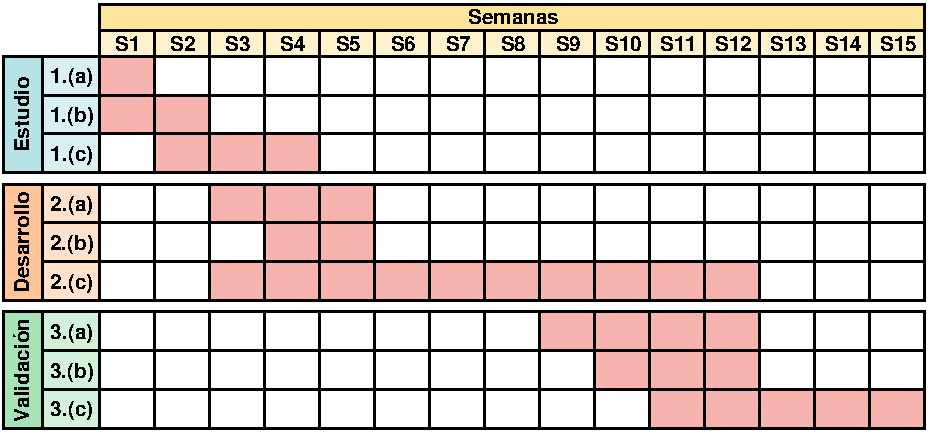
\includegraphics[width=.8\linewidth]{imagenes/investigacion/carta_gantt.pdf}
    \caption{Carta Gantt para el semestre Otoño 2025}
    \label{fig:Gantt}
\end{figure}

\section{Trabajo adelantado}

En lo que respecta al trabajo realizado durante el semestre del curso de “Introducción al Trabajo de Título” (CC6907), este se enfocó principalmente en investigar qué estrategias utilizó el INE para la publicación de los datos del censo de 2017, junto con cuales características tienen los datos, más específicamente, qué técnicas de privatización de datos utilizan y cómo se etiquetan los datos entre cuasi-identificadores, datos sensibles y datos no sensibles. También se indagó en qué restricciones legislativas tiene tal institución para publicar información.

Por otro lado, también se investigó en mayor profundidad el censo de Estados Unidos del año 2020, en particular, acerca de cómo utilizaron el algoritmo “TopDown” para aplicar privacidad diferencial a los datos y cómo funciona tal algoritmo. De manera similar al INE, también se revisó qué restricciones o condiciones tiene su oficina censal para publicar tales datos con el objetivo de poder comparar el proceso chileno con el estadounidense.

\subsection{Censo de Población y Viviendas de Chile 2017}

El Censo de Población y Viviendas de Chile de 2017 recabó información de 17.574.003 personas y 6.499.574 viviendas~\cite{DatosCenso2017}. Estos datos son clave para la planificación de políticas públicas y la toma de decisiones, pero su publicación debe equilibrar las obligaciones de transparencia con la protección de la privacidad establecida por la Ley de Protección de Datos Personales. A continuación, se analizarán las preguntas realizadas y datos de este censo.

En los microdatos publicados, además de los datos asociados a la vivienda y población, se añade la información geográfica acerca de donde se censó tal persona en particular. Tal valor llega hasta un nivel de agregación de la zona o localidad a la cual pertenece la vivienda censada. No se da el valor específico de la dirección de la vivienda para proteger la privacidad. En la figura \ref{fig:division_geografica_chile} se puede apreciar cómo el INE divide el territorio en divisiones más granulares.

\begin{figure}[H]
    \centering
    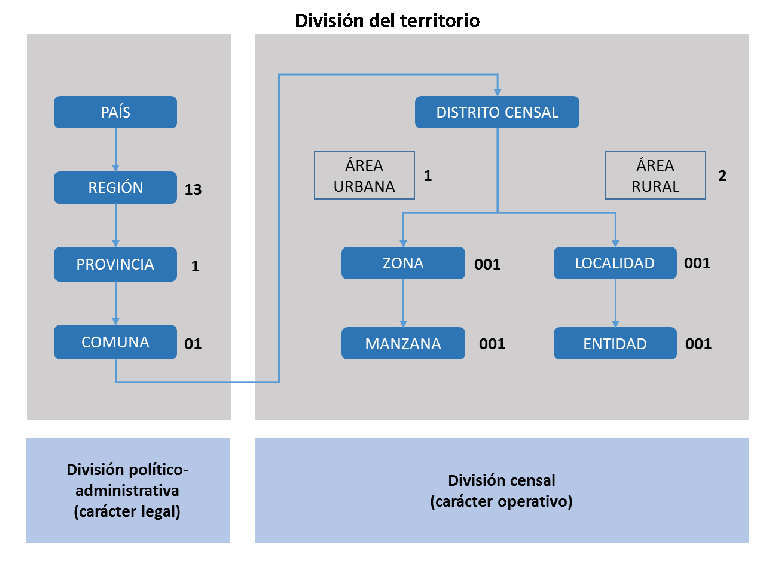
\includegraphics[width=\textwidth]{imagenes/investigacion/division_censal.pdf}
    \caption{División del territorio por el INE para el censo~\cite{INE2017}}
    \label{fig:division_geografica_chile}
\end{figure}

El censo de personas incluye 15 preguntas principales y 4 subpreguntas, sumando 19 en total. Por su parte, el censo de viviendas contiene 6 preguntas, de las cuales 2 tienen subpreguntas. Este volumen de información, aunque útil para diversos fines, aumenta las oportunidades para que un atacante pueda vincular los datos con información auxiliar e identificar a una persona.

Para garantizar la privacidad de los datos recopilados, es importante clasificar la información según su nivel de sensibilidad:

\begin{itemize}
    \item \textbf{Cuasi-identificadores:} Datos que individualmente no identifican a una entidad, pero que de manera colectiva pueden hacerlo, por ejemplo, la comuna de residencia, género y edad.
    \item \textbf{Datos sensibles:} Información cuya divulgación podría generar discriminación o perjuicios a una entidad, como la religión o el estado de salud.
    \item \textbf{Datos no sensibles:} Información general que no está asociada a riesgos de privacidad, como por ejemplo el material de un suelo.
\end{itemize}

Ahora, a continuación se listarán cada una de las preguntas que son incluidas en los microdatos con una descripción de a que se refiere si es necesario. También se define su respectiva clasificación y se incluye la información geográfica. En otras palabras, se analizarán y clasificarán los microdatos. 

\subsubsection*{Clasificación de microdatos del censo de viviendas}

Las columnas en los microdatos están escritas de manera abreviada, se explicitará tal notación para facilitar la comprensión de los microdatos a futuro.

\begin{itemize}
    \item Identificación geográfica hasta el nivel de localidad (\textbf{ID\_ZONA\_LOC}).
    Se considera como \textbf{cuasi-identificador}.
    \item Pregunta 1 (\textbf{P01}). Indica el tipo de vivienda, es decir, si es una casa, un departamento, una vivienda móvil, entre otras opciones. Se considera como \textbf{cuasi-identificador}.
    \item Pregunta 2 (\textbf{P02}). Indica si la vivienda está ocupada o desocupada, explicitando cuando está desocupada si es por que los moradores están ausentes, porque esta en venta o porque es una vivienda de temporada o vacaciones. Este dato se considera como \textbf{sensible} porque una persona podría aprovecharse de esta información para ver si una vivienda esta vacía para ejecutar un delito, como el de un hurto.
    \item Pregunta 3 (\textbf{P03A, P03B y P03C}). Indica el material con el cual estan hechas las paredes, la cubierta del techo y el piso respectivamente. Se considera como datos \textbf{no sensible}. % Revisar esta desición.
    \item Pregunta 4 (\textbf{P04}). Indica la cantidad de habitaciones que se usan como dormitorio. Se considera como \textbf{no sensibles}.
    \item Pregunta 5 (\textbf{P05}). Indica de donde proviene principalmente el agua que se usa en la vivienda. Se considera como \textbf{no sensible}.
    \item Pregunta 6 (\textbf{CANT\_PER}). Identifica la cantidad de personas que pasaron la noche en esa vivienda en particular el día que fue censada. Esta pregunta se subdivide en 4, pero en los microdatos únicamente se indica la cantidad de persona. Se considera como dato \textbf{no sensible}.
\end{itemize}

De lo anterior, se puede notar que no existen muchos datos que faciliten hacer un ataque de asociación de registro, sin embargo, al haber un dato sensible es importante preocuparse de que efectivamente no se pueda realizar esto. 

También cabe notar que si una vivienda está desocupada, esta no puede ser censada, pues no habría una persona capaz de responder las preguntas. El cuestionario del censo considera esta situación y no son respondidas las preguntas posteriores a la 2 si esto sucede. La figura \ref{fig:flujoVivienda} muestra el diagrama de flujo que sigue el censo de viviendas.

\begin{figure}[H]
    \centering
    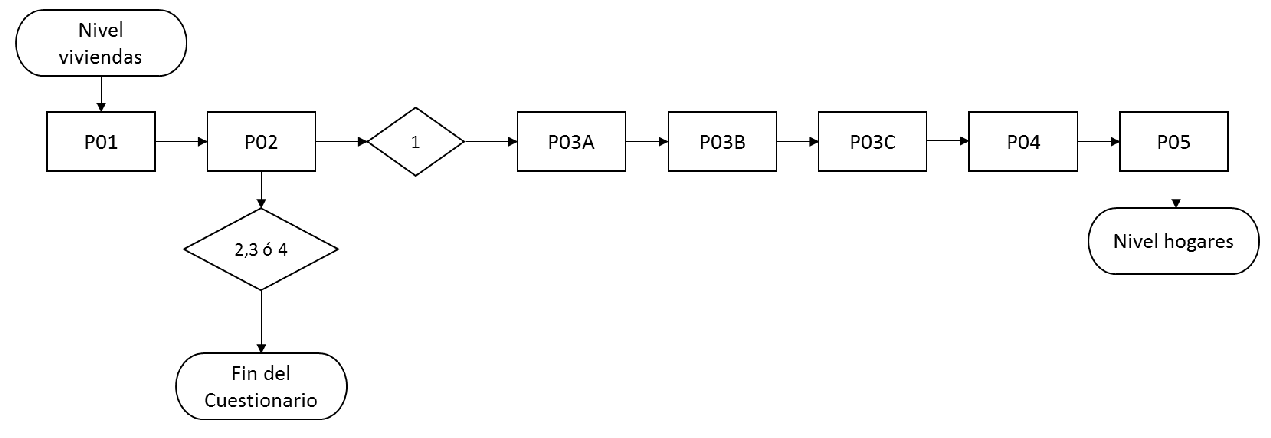
\includegraphics[width=\linewidth]{imagenes/investigacion/flujo_censo_viviendas.pdf}
    \caption{Diagrama de flujo del Censo de Vivienda~\cite{INE2017}}
    \label{fig:flujoVivienda}
\end{figure}

\subsubsection*{Clasificación de microdatos del censo de población}

De la misma manera que para el censo de viviendas, se incluirá la notación utilizada en los microdatos y la información geográfica presente en estos.

\begin{itemize}
    \item Identificación geográfica hasta el nivel de localidad (\textbf{ID\_ZONA\_LOC}).
    Se considera como \textbf{cuasi-identificador}.
    \item Pregunta 7 (\textbf{P07}). Indica la relación de parentesco que se tiene con el jefe de hogar, por ejemplo, hijo, hermano, pareja, entre otros. Se considera como dato \textbf{no sensible}.
    \item Pregunta 8 (\textbf{P08}). Indica el sexo de la persona censada. Se considera como \textbf{cuasi-identificador}.
    \item Pregunta 9 (\textbf{P09}). Indica la edad de la persona, usa como cota superior la edad 100, es decir si una persona tiene más de 100 años se establece como si tuviese 100. Se considera como \textbf{cuasi-identificador}.
    \item Pregunta 10 (\textbf{P10, P10COMUNA y P10PAIS}). Indica si la persona reside habitualmente en la comuna en la fue censada, en caso de que no sea así, se pregunta en que otra comuna o país habita normalmente. Se considera como dato \textbf{cuasi-identificador}.
    \item Pregunta 11 (\textbf{P11, P11COMUNA y P11PAIS}). Indica si en abril de 2012 habitaba en la misma comuna que la pregunta anterior o en otra comuna o país. Se considera como \textbf{no sensible}.
    \item Pregunta 12 (\textbf{P12, P12COMUNA, P12PAIS, P12\_LLEGADA y P12\_TRAMO}). Indica en qué comuna o país habitaba la madre de la persona censada en el momento de su nacimiento. En caso de que haya nacido en otro país se pregunta que año o rango de años llego a Chile. También se considera como datos \textbf{no sensibles}.
    \item Pregunta 13 (\textbf{P13}). Indica si actualmente la persona censada asiste a educación formal. Se considera como dato \textbf{no sensible}.
    \item Pregunta 14 (\textbf{P14}). Indica el curso o año más alto aprobado considerando la respuesta de la pregunta anterior. Se considera como dato \textbf{no sensible}.
    \item Pregunta 15 (\textbf{P15 y P15A}). Especifica que educación formal se refiere la persona censada en los puntos anteriores. Por ejemplo, que tipo de educación media (Científico-Humanista, Técnica profesional, etc...) o que tipo de educación superior (Técnica, Profesional, Magister o Doctorado). La pregunta P15A responde si terminó el nivel de educación declarado. Se considera como dato \textbf{sensible} puesto que una persona podría utilizar este dato, por ejemplo, para discriminar a que personas considerar en un proceso de contratación.
    \item Pregunta 16 (\textbf{P16, P16A y P16\_OTRO}). Indica si la persona censada se considera o no perteneciente a un pueblo originario y especifica a cual en caso afirmativo. Esto se podría considerar como un \textbf{dato sensible}, pues en algunas partes del país existen problemáticas sociales, territoriales, militares y sesgos asociados a pueblos indígenas en especifico. Así, una persona que se considera parte de estos grupos, pero que quiere evitar ser relacionada con estas problemáticas, es probable que quiera mantener de manera privada tal información.
    \item Pregunta 17 (\textbf{P17}). Indica si trabajó o no la semana pasada. Se especifica según corresponda en hasta 6 categorías. Este dato se considera como \textbf{no sensible}.
    \item Pregunta 18 (\textbf{P18}). Indica el rubro al cual se dedica la empresa, institución o actividad independiente en la cuál trabajó la persona censada. Se considera como \textbf{no sensible}.
    \item Pregunta 19 (\textbf{P19}). Indica la cantidad de hijos nacidos vivos que ha tenido una mujer mayor a 15 años. Se considera como dato \textbf{sensible} junto a las siguientes 3 preguntas.
    \item Pregunta 20 (\textbf{P20}). Indica la cantidad de esos hijos que, en el momento de ser censada la madre, siguen estando vivos.
    \item Pregunta 21 (\textbf{P21M y P21A}). Indica el mes y año que nació el último hija o hijo de la madre censada. Estas 3 preguntas permiten inferir cuantos hijos de una madre han fallecido, lo cual es muy probable que quiera ser privatizado por una madre ya que la muerte de un hijo es un evento personal y doloroso, considerado como información altamente sensible desde el punto de vista emocional y social. Esto podría dar lugar a estigmatización o discriminación en ciertos contextos.
\end{itemize}

Considerando la clasificación anterior, se puede notar que para el censo de personas existe una mayor cantidad de datos para una posible reidentificación por parte de un atacante. Además, también existe una mayor presencia de datos sensibles. Esto nuevamente refuerza lo importante que es implementar un mecanismo de privatización de estos datos lo suficientemente fuerte para evitar exponer los datos de las personas del censo. 

Al igual que el censo de viviendas, hay preguntas que no son respondidas por todas las personas. El flujo que sigue este cuestionario es bastante más complejo, por ejemplo, las preguntas posteriores a la 16 no son respondidas si la persona censada es menor a 15 años. En la figura \ref{fig:flujoPersonas} se puede apreciar el diagrama de flujo que sigue el cuestionario del censo de personas.

\begin{figure}[H] % Dejar una hoja aparte
    \centering
    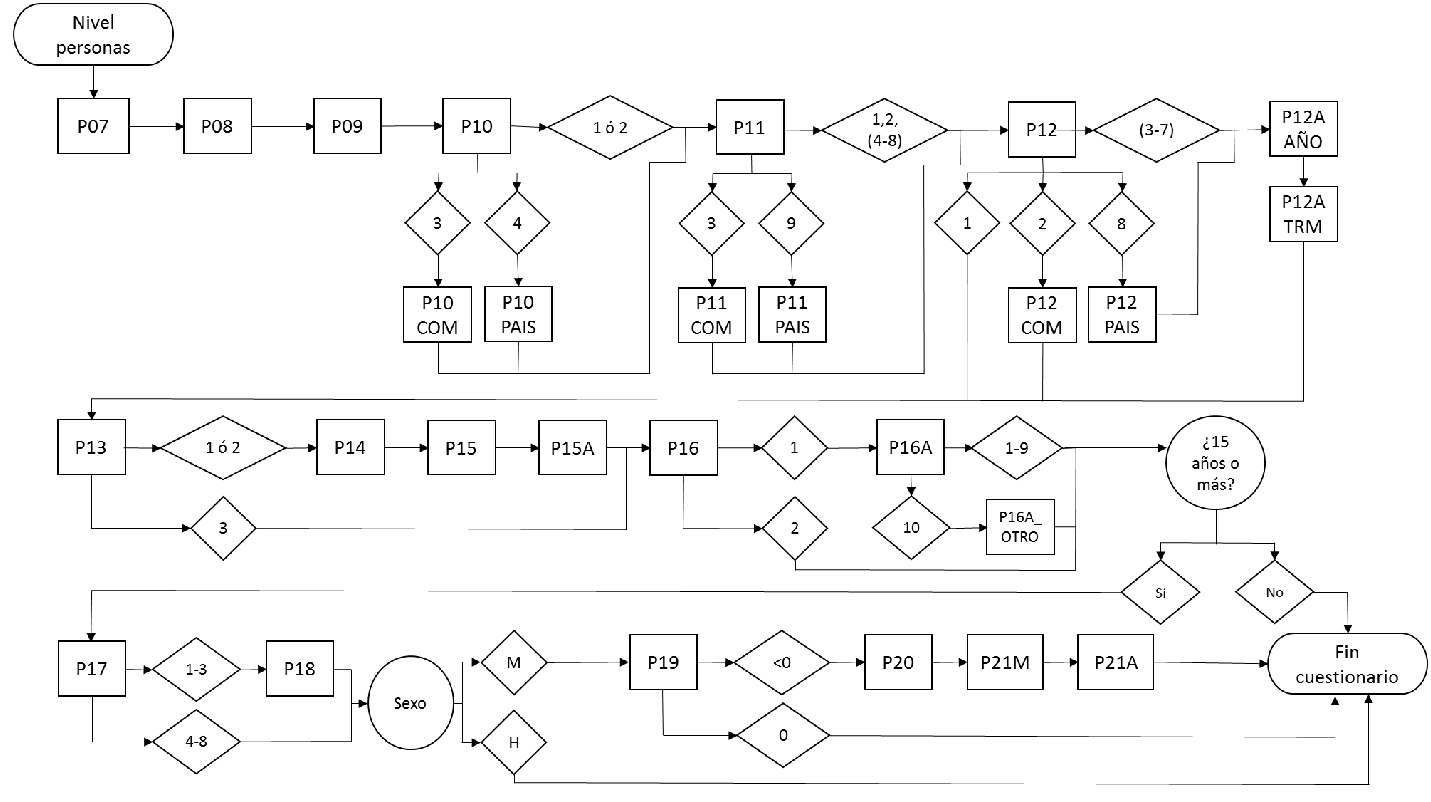
\includegraphics[width=\linewidth]{imagenes/investigacion/flujo_censo_personas.pdf}
    \caption{Diagrama de flujo del Censo de Personas~\cite{INE2017}}
    \label{fig:flujoPersonas}
\end{figure}


\subsection{Métodos de privatización usados en el censo}
El Instituto Nacional de Estadísticas (INE) utiliza diversas técnicas para proteger la confidencialidad de los datos al publicarlos. Sin embargo, la documentación oficial deja de manera ambigua acerca de específicamente cuál es la totalidad de métodos que utilizaron. En particular, respecto a la indeterminación de las bases de datos el INE declara:

\begin{quote}
    \textit{“Para realizar la indeterminación se revisó experiencia internacional, con el fin de tener una mirada general del panorama en torno a la protección de los datos de la población. En estas experiencias se constataron altas restricciones en torno a la protección de los datos, siendo los principales métodos de indeterminación el intercambio de datos, la recodificación de variables y categorías, la restricción del nivel de información geográfica, la entrega de valores determinables como “no disponibles”, el redondeo de datos con límites máximos y mínimos, la entrega solo de muestras de la población y el intercambio aleatorio para muestras pequeñas de hogares similares en áreas cercanas, entre otros”}~\cite{INE2017}. 
\end{quote}



A pesar de lo anterior, el INE sí menciona algunas de las decisiones que tomaron para la indeterminación. Por ejemplo, la decisión de quedarse con un nivel de agregación geográfico a nivel de zona o localidad en vez de manzana o entidad. También se indica que en las manzanas o entidades que presentan 3 personas o menos, se suprimió información relacionada al sexo, edad, pertenencia a pueblos indígenas y migración. Además, se menciona que cuando las manzanas o entidades no cumplen con la restricción de que tengan más de 3 viviendas, entonces se agrupan múltiples manzanas/entidades para lograr una mejor privacidad. 

Por último, el INE menciona también que ciertos datos son agrupados debido a que se forman grupos muy pequeños. Esto incluye a las personas mayores a 100 años, a los países de residencia y pueblos originarios con muy poca presencia y el año de llegada al país.

\subsection{Algoritmo TopDown}

Como se mencionó en la sección de trabajo relacionado, se investigó en mayor profundidad el algoritmo TopDown. Esto debido a que, gracias a los múltiples componentes en común que tiene el censo de Estados Unidos con el de Chile, adaptar tal algoritmo al censo nacional es una alternativa excelente para hacer un mecanismo de privatización con mayores garantías formales debido a la privacidad diferencial. En la figura \ref{fig:TopDown} se puede ver el funcionamiento a grandes rasgos de este.

\begin{figure}[H]
    \centering
    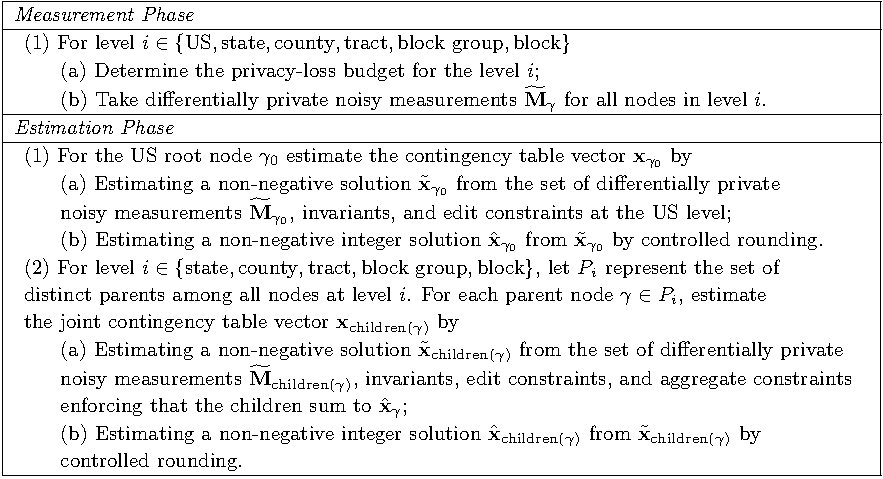
\includegraphics[width=\linewidth]{imagenes/investigacion/TopDown_algorithm.pdf}
    \caption{Extracto del Algoritmo TopDown~\cite{Abowd2022}}
    \label{fig:TopDown}
\end{figure}

Se aprecia que el algoritmo se divide en 2 fases. La primera es la llamada “Measurement Phase” o fase de medición. En esta fase se itera por cada nivel del árbol geográfico, empezando por la raíz. En cada nivel se define un presupuesto de privacidad y se toman mediciones ruidosas para cada nodo del árbol en ese nivel, esto sin considerar ninguna restricción de valores negativos o que exista consistencia entre los valores generados entre un nivel y otro. Luego, en la “Estimation Phase”, fase de estimación o también referida como fase de posprocesamiento, se utiliza lo encontrado en la fase anterior para encontrar una nueva solución. Esta debe parecerse a los valores ruidosos generados y satisfacer todos los invariantes y restricciones. Esto incluye, por ejemplo, que la población a nivel de estado sea la del valor real y que los nodos padres sean consistentes respecto a la agregación de sus nodos hijos.

\subsubsection*{Conceptos preliminares}

Para la generación del ruido se utiliza una distribución Gaussiana discreta $\mathcal{N}_{\Z}(0, \sigma^2)$. En primer lugar, esto se debe a que se publican frecuencias, las cuales son valores enteros no negativos. En segundo lugar, a diferencia de una distribución de Laplace, la Gaussiana es menos “achatada” y tienes “colas” más chicas. Esto quiere decir que la probabilidad de que se generen valores más alejados a la media es menor. Esta decisión es tomada debido a que, para frecuencias de menor magnitud, se busca que sea poco probable que el ruido altere en gran medida el valor real, logrando mantener así mejor la utilidad. Por último, esta distribución satisface privacidad diferencial aproximada y también privacidad diferencial concentrada~\cite{NEURIPS2020_b53b3a3d}. 

En lo que respecta al uso de la privacidad diferencial, el algoritmo TopDown emplea el mecanismo de “zero concentrated differential privacy (zCDP)”. Este pertenece al grupo de mecanismos de privacidad diferencial aproximada, que, a diferencia de la privacidad diferencial tradicional, utiliza dos parámetros: un presupuesto de privacidad $\epsilon$ y una probabilidad de fallo $\delta$. Este enfoque relaja las condiciones de privacidad al permitir un $\epsilon$ más pequeño, introduciendo a cambio una probabilidad $\delta$ de que no se cumpla la desigualdad de privacidad asociada y se rompa la privacidad diferencial~\cite{near_abuah_2021}. 

La zCDP, en particular, conecta con la privacidad diferencial aproximada al utilizar un único parámetro $\rho$, el cual puede ser convertido en $(\epsilon, \delta)$ a través de la siguiente ecuación: 

$$\epsilon = \rho + 2\sqrt{\rho \log(1/\delta)}$$

Este mecanismo simplifica el manejo del presupuesto de privacidad y satisface las garantías de privacidad establecidas por $(\epsilon, \delta)$-DP. Considerando esto, cuando se define un presupuesto de privacidad para cada nivel del árbol geográfico, se refiere a que se establece un $\rho$ para cada nivel del árbol y no un $\epsilon$.

\subsubsection*{Algoritmo}
 
Ahora, tras aclarar estos conceptos se considerará el diagrama de la figura \ref{fig:TopDown_diagramm_example} para aterrizar los distintos conceptos del algoritmo. Este muestra un árbol que representa un ejemplo de jerarquización de la Universidad de Chile. Las tablas de contingencia o histogramas al costado de cada nodo muestran la frecuencia de hombres y mujeres. Los valores que están en azul representan un ejemplo del valor real. Se puede notar que la agregación de las tablas de contingencia de los nodos hijos suman a los del nodo padre para los valores reales. Por otro lado, en color rojo, se tiene el valor ruidoso que sería generado tras agregarle ruido en la fase de medición del algoritmo. Aquí se puede notar que la agregación de las mediciones ruidosas no son consistentes con las mediciones del nodo padre. Además, se puede ver que en el nodo de obstetricia, el valor ruidoso de la frecuencia de hombres quedó con un valor negativo de -1, esto es posible dada la aleatoriedad y la no imposición de restricciones en la fase de medición del algoritmo.

\begin{figure}[H]
    \centering
    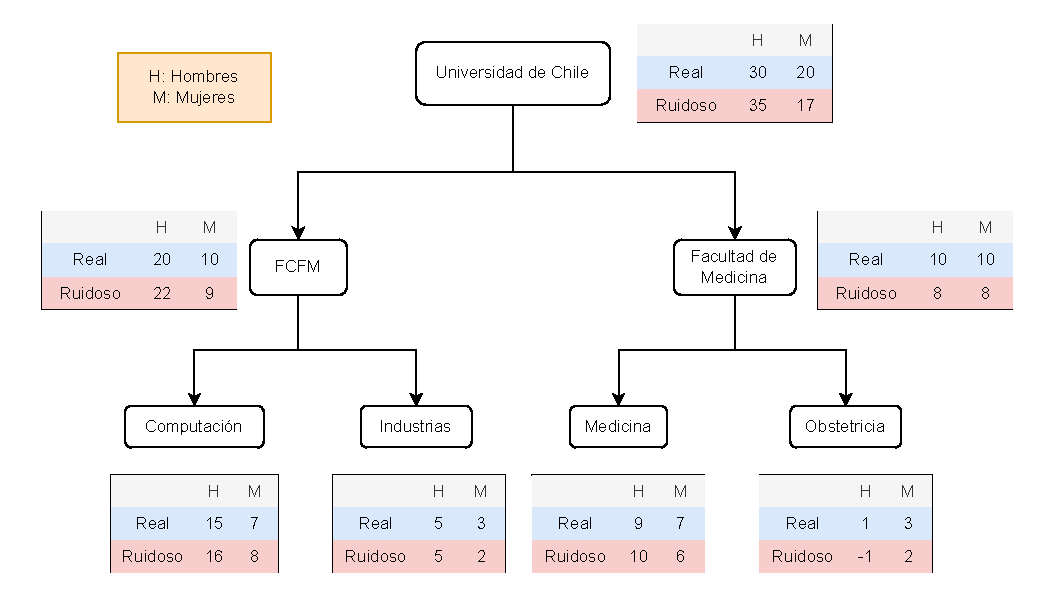
\includegraphics[width=\linewidth]{imagenes/investigacion/TopDown_dummy_example.pdf}
    \caption{Árbol jerárquico de ejemplo con frecuencias reales y ruidosas}
    \label{fig:TopDown_diagramm_example}
\end{figure}

A continuación, utilizaremos y explicaremos la notación empleada en~\cite{Abowd2022} para entender el algoritmo de la figura \ref{fig:TopDown} con el ejemplo de la figura \ref{fig:TopDown_diagramm_example}. 

Primero, denotaremos el arreglo $\rho$ = [0.25, 0.5, 1] como el que contiene los presupuestos de privacidad asociados a cada nivel del árbol, empezando por la raíz. Se usa un presupuesto menor para la raíz ya que la magnitud de las frecuencias es mayor, en cambio, para nodos más cercanos a las hojas, cada vez es necesario tener mayor precisión a la hora de consultar los datos, lo que hace necesario utilizar un presupuesto mayor.

También se representa el árbol con el símbolo $\Gamma$, donde su raíz es $\gamma_{0}$ y los nodos del árbol $\gamma \in \Gamma$. Para referirse al conjunto de nodos hijos de un nodo $\gamma$ se utilizará $\mathit{children(\gamma)}$. Por ejemplo, $\mathit{children(\gamma_{0})} = \{\gamma_{FCFM}, \gamma_{FdM}$\}. A las hojas de un nodo se le llamarán $\mathit{leaves(\gamma)}$ y al padre de un nodo $\mathit{parent(\gamma)}$. Esta notación será relevante cuando se presenten ecuaciones.

También se comprimen los microdatos reales de una matriz \(A \in \mathbb{Z}^{n \times k}\) a una tabla de contingencia o vector $x$.
 El largo de tal vector depende de qué atributos se consideren para su generación. En este caso podemos considerar todos los valores distintos de los datos, los cuales son:

\begin{itemize}
    \item \textbf{Departamentos.} 4 posibilidades: las hojas del árbol.
    \item \textbf{Sexo.} 2 posibilidades: hombre o mujer.
\end{itemize}


 Notemos que no se considera los 7 nodos del árbol debido a que se pueden ir agregando los hijos, partiendo de las hojas, para formar los valores internos del árbol. Puede pensarse como el equivalente a que una columna entregue la comuna, y que a partir de esta se puedan agregar para obtener las regiones y el país. Por otro lado, en la práctica, la magnitud de todas las posibles permutaciones entre los valores distintos de todas columnas de los microdatos haría que el costo algorítmico se dispare considerablemente, por lo que se deberá escoger un subconjunto de atributos con los que trabajar.
 
Ahora, la cantidad de posibles combinaciones sería $c = 4 * 2 = 8$ debido a que hay 2 posibles sexos y 4 posibles geografías en las hojas del árbol. De manera similar, para un $\gamma_i$ dado se tiene que $c^* = 2$, ya que al fijar $\gamma_i$ no se considera la geografía para el cálculo de $c$. 

Considerando estas definiciones, ahora el vector $x$ que contiene los valores reales tiene un largo $c$. Donde el vector puede asumirse que esta ordenado de cierta manera para que describa en su totalidad a la tabla de contingencia. Por ejemplo, podría definirse el vector:

$$x = [15, 7, 5, 3, 9, 7, 1, 3]$$

Donde el orden se consigue al iterar por las hojas del árbol, de izquierda a derecha, y obteniendo las frecuencias de hombres y mujeres en cada nodo. Así el primer 15 corresponde a la cantidad de hombres en el Departamento de Ciencias de la Computación (DCC), el primer 7 a la cantidad de mujeres, el primer 5 a la cantidad de hombres del Departamento de Ingeniería Industrial (DII), y así sucesivamente. De igual forma, podemos denotar como $x_{\gamma}$ como el vector para un nodo $\gamma$ en específico. Por ejemplo, para $\gamma = $ FCFM, se tendría el vector $x_{\gamma} = [20, 10]$ de largo $c^* = 2$.

Junto a esto, se debe definir un conjunto de consultas lineales $Q$ que se harán sobre $x$, tal que el producto matricial $Qx$ entregue los resultados de tales consultas. La representación será $Q \in \{0, 1\}^{a \times c}
$ para el árbol, o bien, $Q_{\gamma} \in \{0, 1\}^{a \times c^*}$ para un nodo $\gamma$ fijo. Donde $a$ representa la cantidad de consultas que se harán.

Considerando lo anterior, para el ejemplo podemos definir la matriz $Q_{\gamma}$ como: 

$$
Q_{\gamma} = \begin{bmatrix}
    1 & 1 \\
    1 & 0 \\
    0 & 1
\end{bmatrix}
$$

Donde la primera fila representa la consulta por el total de personas, la segunda por el total de hombres y la tercera por el total de mujeres para un nodo $\gamma$ en especifico. 

Esto se puede generalizar para el árbol en su totalidad, se podría obtener las mismas consultas al concatenar las matrices $Q_{\gamma}$ del nivel inferior de manera horizontal, o bien, se podría rescatar la misma consulta del nivel inferior al concatenar de manera vertical y rellenando con ceros de manera horizontal. Haciendo estas 2 operaciones se obtiene una matriz que representa todas las consultas del árbol. Por ejemplo, para el árbol $\Gamma_{FCFM}$, tendríamos:

$$
Q_{\Gamma_{FCFM}} = \begin{bmatrix}
    1 & 1 & 1 & 1 \\
    1 & 0 & 1 & 0 \\
    0 & 1 & 0 & 1 \\
    1 & 1 & 0 & 0 \\
    1 & 0 & 0 & 0 \\
    0 & 1 & 0 & 0 \\
    0 & 0 & 1 & 1 \\
    0 & 0 & 1 & 0 \\
    0 & 0 & 0 & 1 
\end{bmatrix}
$$

Donde la primera fila es la consulta por el total de personas a nivel FCFM, la segunda la cantidad de hombres, la tercera la cantidad de mujeres, la cuarta la cantidad de personas del DCC, la quinta la cantidad de hombres en el DCC, y así sucesivamente. 

Considerando esto, se puede representar el vector con el resultado de las consultas simplemente como $Qx$. Por ejemplo, para el nodo $\gamma_{DCC}$, tendriamos:

$$
\begin{bmatrix}
    1 & 1 \\
    1 & 0 \\
    0 & 1
\end{bmatrix}
\begin{bmatrix}
    15 \\ 
    7
\end{bmatrix}
=
\begin{bmatrix}
    22 \\
    15 \\
    7
\end{bmatrix}
$$

Finalmente, teniendo en consideración toda esta notación, podemos definir el vector que agrega ruido a los resultados de los consultas como $y$. Donde $y \sim \mathcal{N}_{\Z}(0, \sigma^2)$ debido a lo explicado en la sección anterior.

Así el vector que contiene los valores ruidosos se puede denotar como $\widetilde{M} = Qx + y$. En particular, en el ejemplo; $\widetilde{M}_{DCC} = 
\begin{bmatrix}
    24 \\
    16 \\
    8
\end{bmatrix}
$.

\subsubsection*{Fase de Medición}

Teniendo lo anterior en cuenta, la fase de medición es simple. Se itera por cada nivel del árbol geográfico, en este caso, a nivel universidad, luego a nivel de facultades y finalmente a nivel departamentos. En cada nivel se asigna un presupuesto de privacidad, que este caso es el arreglo $\rho =$ [0.25, 0.5, 1] que definimos anteriormente. Luego, se toman mediciones ruidosas para cada nodo de ese nivel, es decir, se toma la tabla de contingencia $x_{\gamma}$, se hacen las consultas $Q_{\gamma}x_{\gamma}$ y se le agrega el ruido $y_{i}$ considerando el presupuesto $\rho_i$. Obteniendo de esta manera, en cada nodo del árbol, un vector $\widetilde{M}_{\gamma} = Q_{\gamma}x_{\gamma} + y_i$ que es el que esta representado en rojo en la figura \ref{fig:TopDown_diagramm_example}.

\subsubsection*{Fase de Estimación}

Una vez terminada la fase de medición, se empieza la fase de estimación o posprocesamiento. Esta itera de manera parecida a la fase anterior, pero en cada nivel lo que hace es estimar una solución que se parezca “lo más posible” a cada $\widetilde{M}_{\gamma}$, pero que satisfaga invariantes de igualdad, desigualdad y sea consistente con los nodos del padre. 

Los invariantes están relacionados a requisitos de publicación. Es en este punto donde se impone que la población estatal tiene que ser publicada con el valor real, esto debido a las políticas de transparencia del mandato constitucional~\cite{Abowd2022}. También, en el caso del censo de viviendas, la cantidad de personas en un establecimiento debe ser mayor que 0. Además es aquí cuando se preocupa que el árbol sea consistente en sus valores, es decir, que la agregación de los nodos hijos sumen a los del padre considerando las soluciones encontradas.

Ahora, por temas de complejidad computacional, en cada nodo se divide la estimación en encontrar 2 estimaciones distintas. En primer lugar, se utiliza un estimador de mínimos cuadrados para encontrar una solución real no negativa que cumpla los invariantes, para luego, utilizar un estimador de redondeo para discretizar la solución. 

Primero, el nodo raíz se procesa por separado, esto debido a que no tiene padre con el cual ser consistente. Entonces, se busca primero una solución real no negativa que cumpla los invariantes a través de una estimación de mínimo cuadrados. Se plantea el siguiente problema de optimización:

\begin{equation}
    \begin{aligned}
    \tilde{x} \leftarrow \arg\min_{x_{\gamma}} &\left( (Qx_{\gamma} - \widetilde{M}_{\gamma})^\top W (Qx_{\gamma} - \widetilde{M}_{\gamma}) \right) \\
    &\text{sujeto a:} \\
    &x_{\gamma} \geq 0, \\
    &C^{eq} x_{\gamma} = c^{eq}, \\
    &C^u x_{\gamma} \leq c^u
    \end{aligned}
\end{equation}

De este problema, la matriz $W$ representa una matriz de pesos que contiene la varianza inversa de las variables aleatorias diferencialmente privadas a lo largo de su diagonal~\cite{Abowd2022}. También, se da cuenta que lo que se busca encontrar es, entre todos los posibles vectores o tablas de contingencias $x_{\gamma}$ no negativos que satisfacen las restricciones planteadas, aquel que tiene los resultados a las consultas $Q$ más parecidos a las respuestas ruidosas $\widetilde{M}_{\gamma}$ calculadas en la fase de estimación.

Luego, la primera restricción es la que impone que todos los valores deben ser no negativos. La segunda restricción impone que se cumplan los invariantes de igualdad, como por ejemplo, que la población a nivel sea efectivamente la real. En este caso, podemos suponer que la cantidad de personas a nivel facultad debe ser transparente y publicar el valor real. Así, $c^{eq} = \begin{bmatrix}
    30 \\
    20
\end{bmatrix}$ podría representar el vector con los valores reales, en este caso.

Sin embargo, a nivel de la raíz esto aun no tiene mucho sentido, ya que al estar fijando el nodo, la tabla de contingencia de la raíz $x_{\gamma_0}$ no tiene información de las personas por facultad, sino solo a nivel de universidad. Equivalentemente en Estados Unidos, solo se tiene la información a nivel nacional. Por lo que tal valor de $c^{eq}$ será útil cuando se vaya a un nivel del árbol más bajo. No obstante, en la práctica se pueden definir otras restricciones de igualdad si los datos lo requieren.

Luego, $C^{eq}$ sería parecida a $Q$, ya que es la matriz que transforma $x_{\gamma}$ en $c^{eq}$, en otras palabras, consulta $x_{\gamma}$ para transformarlo en el vector $c^{eq}$. La misma explicación aplica a la última restricción, la cual tiene que ver con las desigualdades. Un ejemplo de esto es que un establecimiento no puede tener 0 personas en Estados Unidos en el censo de viviendas. Así, $C^{u}$ y $c^u$ se construyen de manera similar a $C^{eq}$ y $c^{eq}$.

En este punto del algoritmo en el cual se esta rompiendo la privacidad diferencial, ya que se están transformando los resultados ruidosos a unos datos más convenientes para la publicación. Es más, al imponer las restricciones de igualdad, se esta encontrando una solución que no utiliza privacidad diferencial para los datos expuestos en $c^{eq}$. Podría entenderse que para estos valores se le asigna un presupuesto de privacidad infinito~\cite{Abowd2022}, es decir, optando por la utilidad máxima a cambio de sacrificar la privacidad.

Por otro lado, podría argumentarse que, por las propiedades de posprocesamiento de la privacidad diferencial, esto no es cierto. Esto es una discusión que no se abordará actualmente, pero durante el próximo semestre podría ser interesante investigar e indagar al respecto.

Una vez resuelto este problema, se obtiene entonces un $\tilde{x}$ que representa una solución real no negativa que cumple con las restricciones, pero debido a que se publican frecuencias, ahora se necesita recurrir a un estimador de redondeo para discretizar la solución.

De manera similar para el cálculo de la solución de $\tilde{x}$, se plantea un problema de optimización para encontrar la solución no negativa entera que más se parezca a $\tilde{x}$:

\begin{equation}
    \begin{aligned}
        \hat{x}_{\gamma} \leftarrow &\lfloor \tilde{x}_{\gamma} \rfloor + \hat{y}, \\
        &\hat{y} = \arg\min_{y} \left( 1^\top \big|\tilde{x}_{\gamma} - \big( \lfloor \tilde{x}_{\gamma} \rfloor + y \big) \big| \right) \\
        &\text{sujeto a:} \\
        &y_i \in \{0, 1\} \text{ para } y_i \text{ un elemento de } y; \\
        &C^{eq} \big( \lfloor \tilde{x}_{\gamma} \rfloor + y \big) = c^{eq}; \\
        &C^u \big( \lfloor \tilde{x}_{\gamma} \rfloor + y \big) \leq c^u.
    \end{aligned}
\end{equation}

De esto se puede notar que, $\hat{x}_{\gamma}$ sería la solución final para el nodo raíz, la cual cumple con todas las restricciones. Luego, la expresión $\lfloor \tilde{x}_{\gamma} \rfloor + \hat{y}$ hace referencia a que, de la solución encontrada en el paso anterior, se trunca todos los valores y se les suma un valor $y_i \in  \{0, 1\}$, discretizando la solución. Se debe notar que el valor que es encontrado en esta estimación no es $\tilde{x}_{\gamma}$, sino que es el valor $\hat{y}$ que dice a que elementos de $\lfloor \tilde{x}_{\gamma} \rfloor$ se les suma 1 o no. Luego, las restricciones son las esperables, ya que son idénticas al estimador de mínimos cuadrados considerando que $\lfloor \tilde{x}_{\gamma} \rfloor + y$ representa la solución que se encontrará con esta segunda estimación.

Con esto completado, finalmente el algoritmo entra en un último paso, el cual es iterar por todos los niveles del árbol exceptuando la raíz. Donde, para cada nodo $\gamma$ de un nivel del árbol dado, se resuelven los mismos problemas de estimación, solo que esta vez se agrega una condición adicional; que los nodos sean consistentes con las soluciones calculadas por su padre. Para esto, es más sencillo pensar que se itera por los nodos padre $\gamma \in P_i$, donde $P_i$ es el conjunto que representa a todos los nodos padres del nivel $i$ del árbol, y se calcula la tabla de contingencia conjunta $x_{\mathit{children}(\gamma)}$. 

Se puede entender $x_{\mathit{children}(\gamma)}$ como el resultado de apilar los valores de $x_{\mathit{child}}$ para $\mathit{child} \in \mathit{children}(\gamma)$. Por ejemplo, considerando el árbol de ejemplo de la figura \ref{fig:TopDown_diagramm_example}:

$$x_{\mathit{children}(FCFM)} = \begin{bmatrix}
    15 \\
    7 \\
    5 \\ 
    3
\end{bmatrix}$$

Luego, de manera similar se puede definir $\widetilde{M}_{\mathit{children}(\gamma)}$ como el mismo vector que $x_{\mathit{children}(\gamma)}$, pero que contiene la agregación de los valores ruidosos de los nodos hijos en vez de los valores reales. Utilizando nuevamente la figura \ref{fig:TopDown_diagramm_example}:

$$\widetilde{M}_{\mathit{children}(FCFM)} = \begin{bmatrix}
    16 \\
    8 \\
    5 \\ 
    2
\end{bmatrix}$$

A continuación se plantean los estimadores modificados teniendo en cuenta la nueva restricción de consistencia:

% Primera ecuación con numeración clara y alineación
\begin{equation} \label{eq:optimization}
    \begin{aligned}
        \tilde{x}_{\mathit{children}(\gamma)} \leftarrow &\arg\min_{x_{\mathit{children}(\gamma)}} 
        \left( \big(Qx_{\mathit{children}(\gamma)} - \widetilde{M}_{\mathit{children}(\gamma)}\big)^\top 
        W \big(Qx_{\mathit{children}(\gamma)} - \widetilde{M}_{\mathit{children}(\gamma)}\big) \right), \\
        &\text{sujeto a:} \\
        &x_{\mathit{children}(\gamma)} \geq 0; \\
        &C^{eq}x_{\mathit{children}(\gamma)} = c^{eq}; \\
        &C^u x_{\mathit{children}(\gamma)} \leq c^u; \\
        &\begin{bmatrix}
            I_{c_*} & I_{c_*} & \cdots & I_{c_*}
        \end{bmatrix} x_{\mathit{children}(\gamma)} = \hat{x}_\gamma. \\
        \\
        \hat{x}_{\mathit{children}(\gamma)} \leftarrow &\lfloor \tilde{x}_{\mathit{children}(\gamma)} \rfloor + \hat{y}, \\
        &\hat{y} = \arg\min_{y} \left( 1^\top \big|\tilde{x}_{\mathit{children}(\gamma)} - \big( \lfloor \tilde{x}_{\mathit{children}(\gamma)} \rfloor + y \big) \big| \right), \\
        &\text{sujeto a:} \\
        &y_i \in \{0, 1\} \text{ para } y_i \text{ un elemento de } y; \\
        &C^{eq} \big( \lfloor \tilde{x}_{\mathit{children}(\gamma)} \rfloor + y \big) = c^{eq}; \\
        &C^u \big( \lfloor \tilde{x}_{\mathit{children}(\gamma)} \rfloor + y \big) \leq c^u; \\
        &\begin{bmatrix}
            I_{c_*} & I_{c_*} & \cdots & I_{c_*}
        \end{bmatrix}
        \big( \lfloor \tilde{x}_{\mathit{children}(\gamma)} \rfloor + y \big) = \hat{x}_\gamma.
    \end{aligned}
\end{equation}

No es difícil notar que las estimaciones son equivalentes a las anteriores, sin embargo, la última restricciones es la que hay que analizar con más cuidado. 

Una restricción de consistencia podría ser, por ejemplo, que la cantidad de hombres de la FCFM coincida con la suma de los hombres en Computación e Industrias. Ahora, para establecer las restricciones de consistencia, se utiliza además de $\tilde{x}_{\mathit{children}(\gamma)}$ la matriz identidad $I_{c_*}$. Tal matriz tiene dimensión $c^*$ debido a que el vector $\tilde{x}_{\mathit{children}(\gamma)}$ tiene dimensión $c^* \times |\mathit{children}(\gamma)|$. Si tomamos como ejemplo el nodo $\gamma = FCFM$ tendremos que $c^* = 2$. Considerando $x_{\mathit{children}(\gamma)}$ como lo expuesto con anterioridad, se concatenan tantas matrices $I_{c_*}$ como nodos hijos tenga $\gamma$. Esto hace que la restricción tenga una matriz de concatenación de identidades de dimensión $c^* \times c^*|\mathit{children}(\gamma)|$ y por lo tanto, el nodo padre tenga dimensión $c^* \times 1$ que es justamente lo que se busca, ya que es la dimensión de su tabla de contingencia. 
Aplicando esto al ejemplo se tiene:


$$\begin{bmatrix}
    I_{c_*} & I_{c_*}
\end{bmatrix}
x_{\mathit{children}(\gamma)}
=
\hat{x}_{\gamma}$$
$$\begin{bmatrix}
    1 & 0 & 1 & 0 \\
    0 & 1 & 0 & 1
\end{bmatrix}
\begin{bmatrix}
    15 \\
    7 \\
    5 \\ 
    3
\end{bmatrix}
=
\begin{bmatrix}
    20 \\
    10
\end{bmatrix}$$

Donde $\hat{x}_{\gamma}$ es exactamente la tabla de contingencia de la FCFM.

Una vez se termina de iterar por todo el árbol, significa que ya se tiene una solución $\hat{x}_{\gamma}$ para cada nodo $\gamma$. Esto es suficiente para dar por terminado el proceso de privatización y luego se pueden tomar todas estas soluciones para publicar los datos según se requiera.

\newpage
\bibliographystyle{babplain}
\bibliography{bibliografia}
\end{document}
